\newif\ifshowsolutions
\showsolutionstrue
\documentclass{article}
\usepackage{listings}
\usepackage{amsmath}
%\usepackage{subfigure}
\usepackage{subfig}
\usepackage{amsthm}
\usepackage{amsmath}
\usepackage{amssymb}
\usepackage{graphicx}
\usepackage{mdwlist}
\usepackage[colorlinks=true]{hyperref}
\usepackage{geometry}
\usepackage{titlesec}
\geometry{margin=1in}
\geometry{headheight=2in}
\geometry{top=2in}
\usepackage{palatino}
\usepackage{mathrsfs}
\usepackage{fancyhdr}
\usepackage{paralist}
\usepackage{todonotes}
\setlength{\marginparwidth}{2.15cm}
\usepackage{tikz}
\usetikzlibrary{positioning,shapes,backgrounds}
\usepackage{float} % Place figures where you ACTUALLY want it
\usepackage{comment} % a hack to toggle sections
\usepackage{ifthen}
\usepackage{mdframed}
\usepackage{verbatim}
\usepackage[strings]{underscore}
\usepackage{listings}
\usepackage{bbm}
\rhead{}
\lhead{}

\renewcommand{\baselinestretch}{1.15}

% Shortcuts for commonly used operators
\newcommand{\E}{\mathbb{E}}
\newcommand{\Var}{\operatorname{Var}}
\newcommand{\Cov}{\operatorname{Cov}}
\newcommand{\Bias}{\operatorname{Bias}}
\DeclareMathOperator{\argmin}{arg\,min}
\DeclareMathOperator{\argmax}{arg\,max}

% do not number subsection and below
\setcounter{secnumdepth}{1}

% custom format subsection
\titleformat*{\subsection}{\large\bfseries}

% set up the \question shortcut
\newcounter{question}[section]
\newenvironment{question}[1][]
  {\refstepcounter{question}\par\addvspace{1em}\textbf{Question~\Alph{question}\!
    \ifthenelse{\equal{#1}{}}{}{ [#1 points]}: }}
    {\par\vspace{\baselineskip}}

\newcounter{subquestion}[question]
\newenvironment{subquestion}[1][]
  {\refstepcounter{subquestion}\par\medskip\textbf{\roman{subquestion}.\!
    \ifthenelse{\equal{#1}{}}{}{ [#1 points]:}} }
  {\par\addvspace{\baselineskip}}

\titlespacing\section{0pt}{12pt plus 2pt minus 2pt}{0pt plus 2pt minus 2pt}
\titlespacing\subsection{0pt}{12pt plus 4pt minus 2pt}{0pt plus 2pt minus 2pt}
\titlespacing\subsubsection{0pt}{12pt plus 4pt minus 2pt}{0pt plus 2pt minus 2pt}


\newenvironment{hint}[1][]
  {\begin{em}\textbf{Hint: }}{\end{em}}

\ifshowsolutions
  \newenvironment{solution}[1][]
    {\par\medskip \begin{mdframed}\textbf{Solution~\Alph{question}#1:} \begin{em}}
    {\end{em}\medskip\end{mdframed}\medskip}
  \newenvironment{subsolution}[1][]
    {\par\medskip \begin{mdframed}\textbf{Solution~\Alph{question}#1.\roman{subquestion}:} \begin{em}}
    {\end{em}\medskip\end{mdframed}\medskip}
\else
  \excludecomment{solution}
  \excludecomment{subsolution}
\fi

\newcommand{\boldline}[1]{\underline{\textbf{#1}}}

% User packages
\usepackage[labelfont=bf]{caption}
\usepackage[labelfont=bf]{caption}
\usepackage[labelfont=bf]{caption}
\usepackage [english]{babel}
\usepackage [autostyle, english = american]{csquotes}
\MakeOuterQuote{"}

% User commands
\setlength{\parindent}{0pt}

\chead{%
  {\vbox{%
      \vspace{2mm}
      \large
      Machine Learning \& Data Mining \hfill
      Caltech CS/CNS/EE 155 \hfill \\[1pt]
      Miniproject 1\hfill
      Released January $28^{th}$, 2017
    }
  }
}

\begin{document}
\pagestyle{fancy}

\section*{1. Introduction}
\medskip
\begin{itemize}

    \item \boldline{Group members} \\
    Eli Sorey \\
    Kun ho (John) Kim

    \item \boldline{Team name} \\
    Stochastic Gradient, Decent

    \item \boldline{Division of labour} \\
    Eli focused on dataset cleaning, feature selection, and feature transformation. (Feature Engineering) Kun ho primarily worked on the model
    selection, model parameter optimization, and ensemble selection methods. (Models and techniques) We delve into the specific of our work in the following sections.

\end{itemize}



\section*{2. Overview}
\medskip
\begin{itemize}

    \item \boldline{Models and techniques tried}
    \begin{itemize}
    \item \textbf{*Ensemble Selection:} Submitted model.
    \item \textbf{Gradient Boosting Machines}
    \item \textbf{Random Forest}
    \item \textbf{Adaptive Boosting}
    \item \textbf{Extra Trees}
    \item \textbf{Support Vector Machines}
    \item \textbf{Artificial Neural Networks}
    \end{itemize}

    \item \boldline{Work timeline}
    \begin{itemize}
    \item \textbf{Day1 - Day4:} Preliminary data-processing \& Broad model selection.
    \item \textbf{Day 4 - Day 8:} Feature engineering \& Single model optimization
    \item \textbf{Day 8 - Day 12:} Ensemble selection \& Final model tuning
    \end{itemize}

\end{itemize}


\newpage


\section*{3. Approach \& Results}
\subsection*{3.1. Overview}
Our team's general pipeline for this competition is outlined in the flow chart below. \\
\begin{figure}[h]
\center
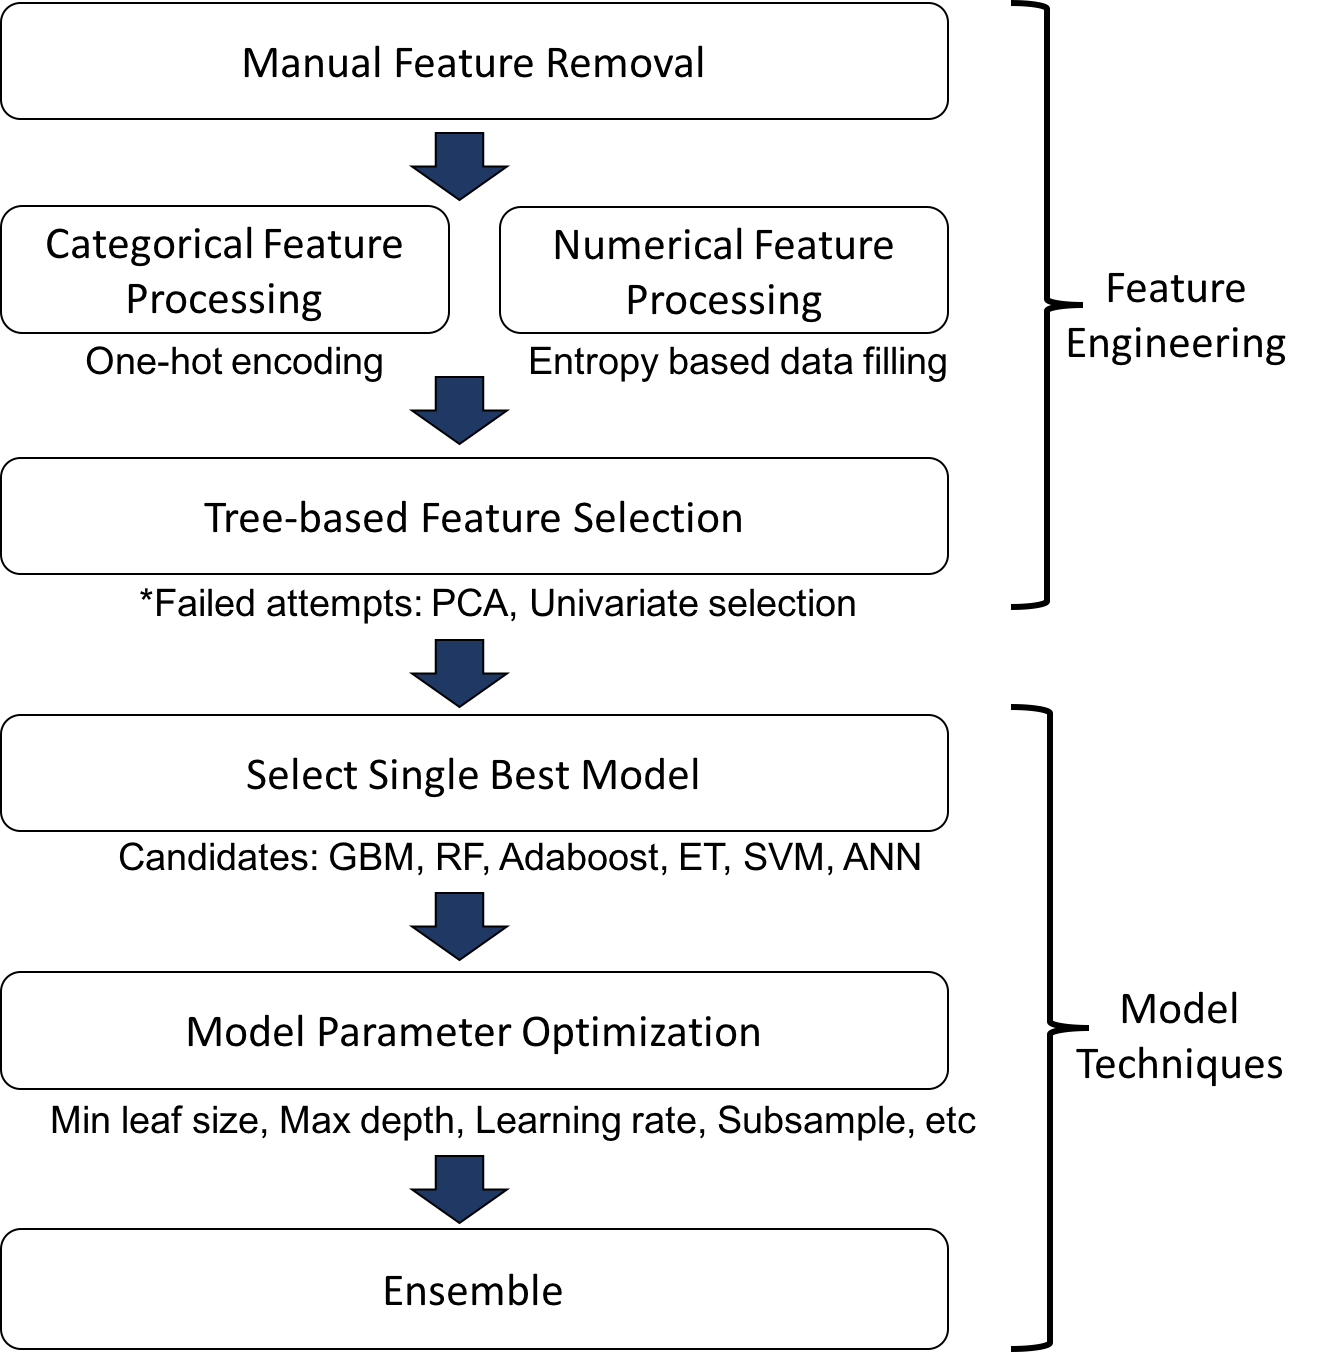
\includegraphics[scale=0.4]{figure1/figure1.png}
\caption{\textbf{Overall pipeline}}
\end{figure}

The feature engineering part of the workflow covers methods of handling categorical features, numerical features, and the feature selection process. The model \& techniques part covers our methods of model selection, parameter
optimization, and stacking/ensemble selecting single models.

\subsection*{3.2. Feature engineering}
The philosophy guiding our approach to feature engineering was to make it as straightforward as possible for our models to pick up on the structures in the data. This was accomplished by reading through the 2008 Codebook describing each of the features. After getting familiar with the features, we applied various transformations to the data to increase the effectiveness of model training.

\subsubsection*{[i]. Manual feature removal}
We sought to remove low-signal features that would either slow down or potentially confuse our models. One thing that immediately stood out after reading through the codebook was the presence of several classes of features that would not be useful to our predictive models. For example,  104 features were marked as 'allocation flags'. Each of these features is associated with another feature, and indicates whether or not the survey participant modified his/her original response. These features were dropped because they do not help in our prediction problem. Other classes of features that were dropped included recodes (redundant features), features that only attained one value on the training set, and features which had responses on less than 1\% of the training set. The effectiveness of this approach was quantified by training a fixed model with fixed parameters on the original data set and the trimmed data set, and then comparing validation set accuracies. The model chosen was sci-kit learn's GradientBoostingClassifier, with 500 estimators and a minimum leaf size of 15 samples. The validation accuracy on the untrimmed data was 0.77490, and the validation accuracy on the trimmed data was 0.778628. This shows that this trimming does in fact improve the quality of the model learned, and while this gain is meager in this case, it stands to be more significant in situations in which we have added more features ourselves (see below). This is because the effect of removing these extraneous features from the data is to decrease the amount of work the model has to do in order to learn a good decision function. We also spent time thinking about how best to deal with negative values. As outlined in the codebook, negative values coincide with non-responses of various kinds. For instance, -1 means that the participant left this question blank, and -3 means the participant refused to answer the question. We decided that differentiating between the different non-responses would be nebulous at best, so we mapped all non-response values to -1.\\

\subsubsection*{[ii]. Categorical feature preprocessing}
Once these unhelpful features were trimmed off of the data, we began looking at ways to make the remaining features more useful to our models. One recurring theme was the presence of features that were numerical encodings of categorical values. For instance, the feature 'PEIO1ICD' was a code for the survey participant's primary occupational industry. Values for this feature ranged from -9 to 9890. It was obvious that this feature had the potential to be predictive, but in its original form, it risked being confusing to our models. This is because a value of 5000 should not be interpreted to be "5 times higher" than a value of 1000; they are simply different categories. To get around this, we used one-hot encodings to represent these features. To do this, we first mapped the given values to their categories (a value of 7970 for 'PEIO1ICD' became 'healthcare service', for instance), and then used the Pandas library to create a new feature for each of the categorical values attained by the original feature. These new features took on value 0 for all participants who did not belong to that category, and value 1 for all those who did - a one-hot encoding of the original data. The original columns were then dropped. We found that this processing improved the performance of our models, both on the validation sets and on the test set.

\subsubsection*{[iii]. Numerical feature preprocessing}
For the numerical (ie, not categorical) features, we were concerned that having a value of -1 for non-responses would confuse the models during their training. Therefore, we decided to replace the negative values with a "fill value". The standard approach to this issue is to replace the non-responses with the mean of the non-negative values attained by the feature of interest. Our concern was that doing this may mislead the prediction model, particularly if the feature carried a high degree of importance for the model. To address this, we devised our own approach for finding fill value, called \textbf{entropy-based value compensation}. Given a feature, we first computed the possible splits that a decision tree could make. We then found the split that minimized the entropy score, corresponding to the choice of split a decision tree would take. Finally, we found the mean of the \textit{higher} entropy side of the split, and used that as our fill value for non-responses within that feature. The logic behind this is that we wanted the fill value to contribute as little as possible to the model's eventual prediction. By using the maximum entropy side, we gave the model as little information as possible through the fill value. Unfortunately, this approach led to decreased model performance, and we reverted to the simple plan of using the mean of the feature.

\subsubsection*{[iv]. Tree-based Feature selection}
The transformations described above ultimately yielded a training set with ~1600 features. At this point, we opted to trim down the number of features before training our models, in the process of feature selection. To do this, we trained an ExtraTreesClassifier from sci-kit learn on the transformed data, and then sorted the features by their importance within the trained model. We then took those features whose importance scores were greater than some fixed constant times the mean of the importance scores. Our goal was to select between 100 and 300 features from the data. Depending on the exact details of our previous feature engineering, the fixed constant was between 1.0 and 3.5. Figure 2 shows the sorted importance scores for features. Note that the majority of importance scores are relatively low; this justifies our approach of selecting the most important features.

\begin{figure}[h]
\center
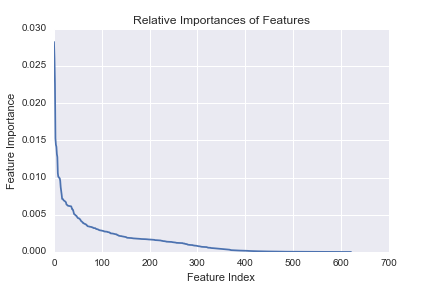
\includegraphics[scale=0.65]{figure5/feature_importances.png}
\caption{\textbf{Sorted feature importance scores}
\textit{Our goal was to capture the most important features and remove the less important ones to make the model's training process easier.}}
\end{figure}

Figure 3 shows the top fifteen features and their importance scores. It is interesting how much the family figures into the model's decisions through features such as HUFAMINC and HRNUMHOU. This suggests that people are motivated to vote not only through their personal attributes, but also by the qualities of their immediate familial circumstances.

\newpage

\begin{figure}[h]
\center
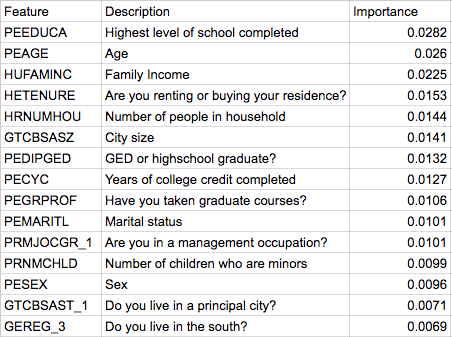
\includegraphics[scale=0.48]{figure5/top_features.png}
\caption{\textbf{Most important features}
\textit{The relative importances shown here were derived from the ExtraTreesClassifier model, as described above.}}
\end{figure}

Figure 4 shows the validation accuracy versus the cutoff threshold for feature selection, evaluated with a baseline model. As described above, a multiplier is given to determine the threshold: if the importance score is greater than or equal to the mean feature score times the multiplier, it is kept. Otherwise, it is discarded. This plot shows that the number of features used for model training has an impact the model performance. Note that the number of features can be too high, or too low.
\begin{figure}[h]
\center
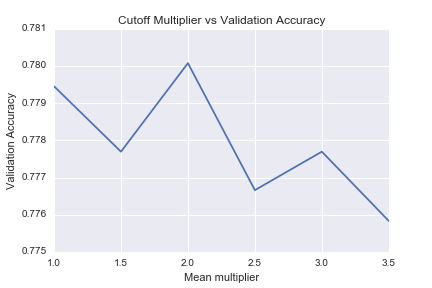
\includegraphics[scale=0.54]{figure5/multiplier_vs_val_acc.png}
\caption{\textbf{Feature selection multiplier vs validation accuracy}
\textit{It is clear that this parameter must be carefully tweaked to achieve an optimal configuration. Note that the model here to evaluate the validation accuracy differed in parameters from the model we used for submissions. We had the best results with ~100 features remaining after feature selection, corresponding to a multiplier of roughly 1.7 in this figure.}}
\end{figure}
The training dataset resulting from the mean cutoff was passed off to a learning algorithm to find the best model. This process is described in the following section 3.3. 

\subsection*{3.3. Model \& Techniques}
\subsubsection*{[i]. Single model selection through cross validation}
After preprocessing the training data, 6 broad model classes(GBM, RF, Adaboost, ET, SVM, ANN) were considered as candidates to determine which achieves the best single-model performance. 5-fold cross validation was performed and the model with the highest validation accuracy was chosen. The following bar graph demonstrates that gradient boosting machines (GBM) performed the best with a validation accuracy of $77.9\%$ (with default parameters).
\begin{figure}[h]
\center
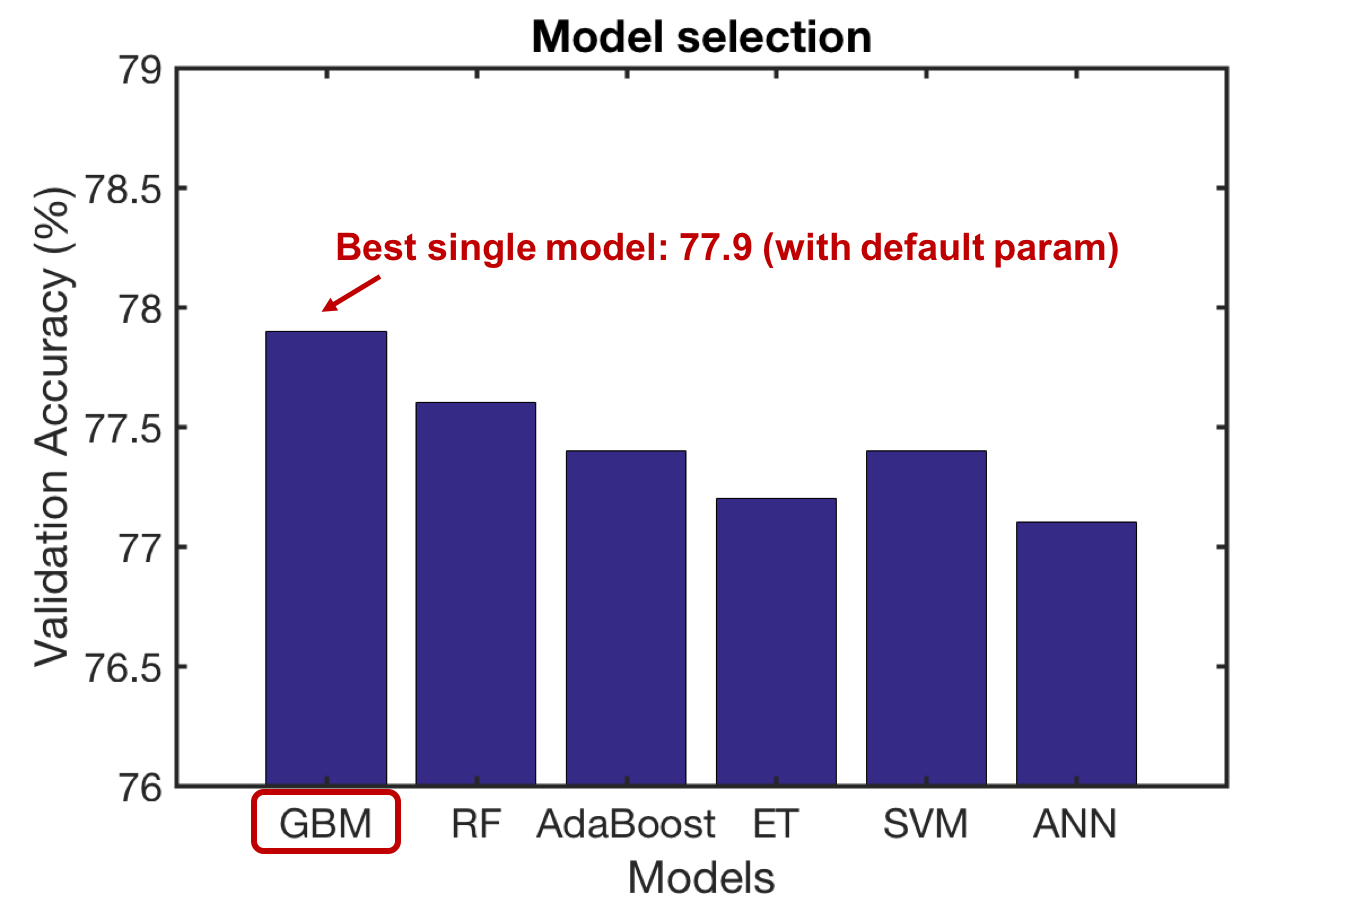
\includegraphics[scale=0.45]{figure2/figure2.png}
\caption{\textbf{Cross validation for single best model selection} \textit{GBM attains the highest accuracy of $77.9\%$ followed by random forests(77.6), Adaboost(77.4), Extra Trees(77.2), Support Vector Machines (77.4), and Artificial Neural Networks (77.1).}}
\end{figure}

Generally, we saw that tree-based non-linear classifiers out-performed linear models such as support vector machines. We attribute this to the fact that demographic features are often only separable by highly non-linear discriminant boundaries. This is in agreement with the fact that the training data projected onto the first two principal components showed no notable separating boundaries. (Hence, our attempt to preprocess the data using principal component eigenvector bases transformation was unsuccessful) This influenced our decision of including more tree-based non-linear classifiers into the pool of models to perform cross validation on. GBMs proved to be a low variance model as it achieved repeatable validation accuracy. (Random forests had relatively higher variance) However, the low variance characteristic made it difficult to enhance the performance of GBMs by only including GBMs in the pool of trained models to ensemble select on. Section 3.3-[iii] will elaborate more on this issue. We now move on to show the results of optimizing GBM model parameters.

\newpage

\subsubsection*{[ii]. Parameter optimization for GBM}
After selecting Gradient Boosting Machines(GBM) as the single best model, we sought to optimize the boosting base model (decision tree) parameters as well as the boosting specific parameters. We considered 5 main parameters for optimization: minimum leaf size, maximum height, learning rate, subsample, and number of estimators. Minimum leaf size and maximum height are both decision tree parameters which control the degree of regularization. Moreover, learning rate, subsample, and number of estimators alters the degree of stochasticity in training each base model, the constants involved in the boosting equation, and the number of boosted trees to train. The number of estimators demonstrated no significant impact on the cross validation accuracy beyond 500 trees and thus we omit the plot regarding this parameter. In fig. 4. we show the validation accuracy of the GBM model plotted against the remaining 4 parameters subject to optimization. The optimum parameters were discovered through a grid search function provided by sklearn, which performs cross validation on the full space of possible parameter quadruples (min leaf size, max height, learning rate, sub sample). Here we show the cross validation performance of each parameter separately, while fixing all other parameters to be the optimum values. Due to the slight randomness in the model that the learning algorithm converges to, the maximum cross validation accuracy differs slightly from plot to plot. Since we seek to show quantitative rationale for our choice of the optimum parameters, we deem these plots as sufficient. The overall best parameters chosen for the GBM model were: (min leaf size, max height, learning rate, sub sample) = (15, 3, 0.1, 1).
\begin{figure}[h]
\center
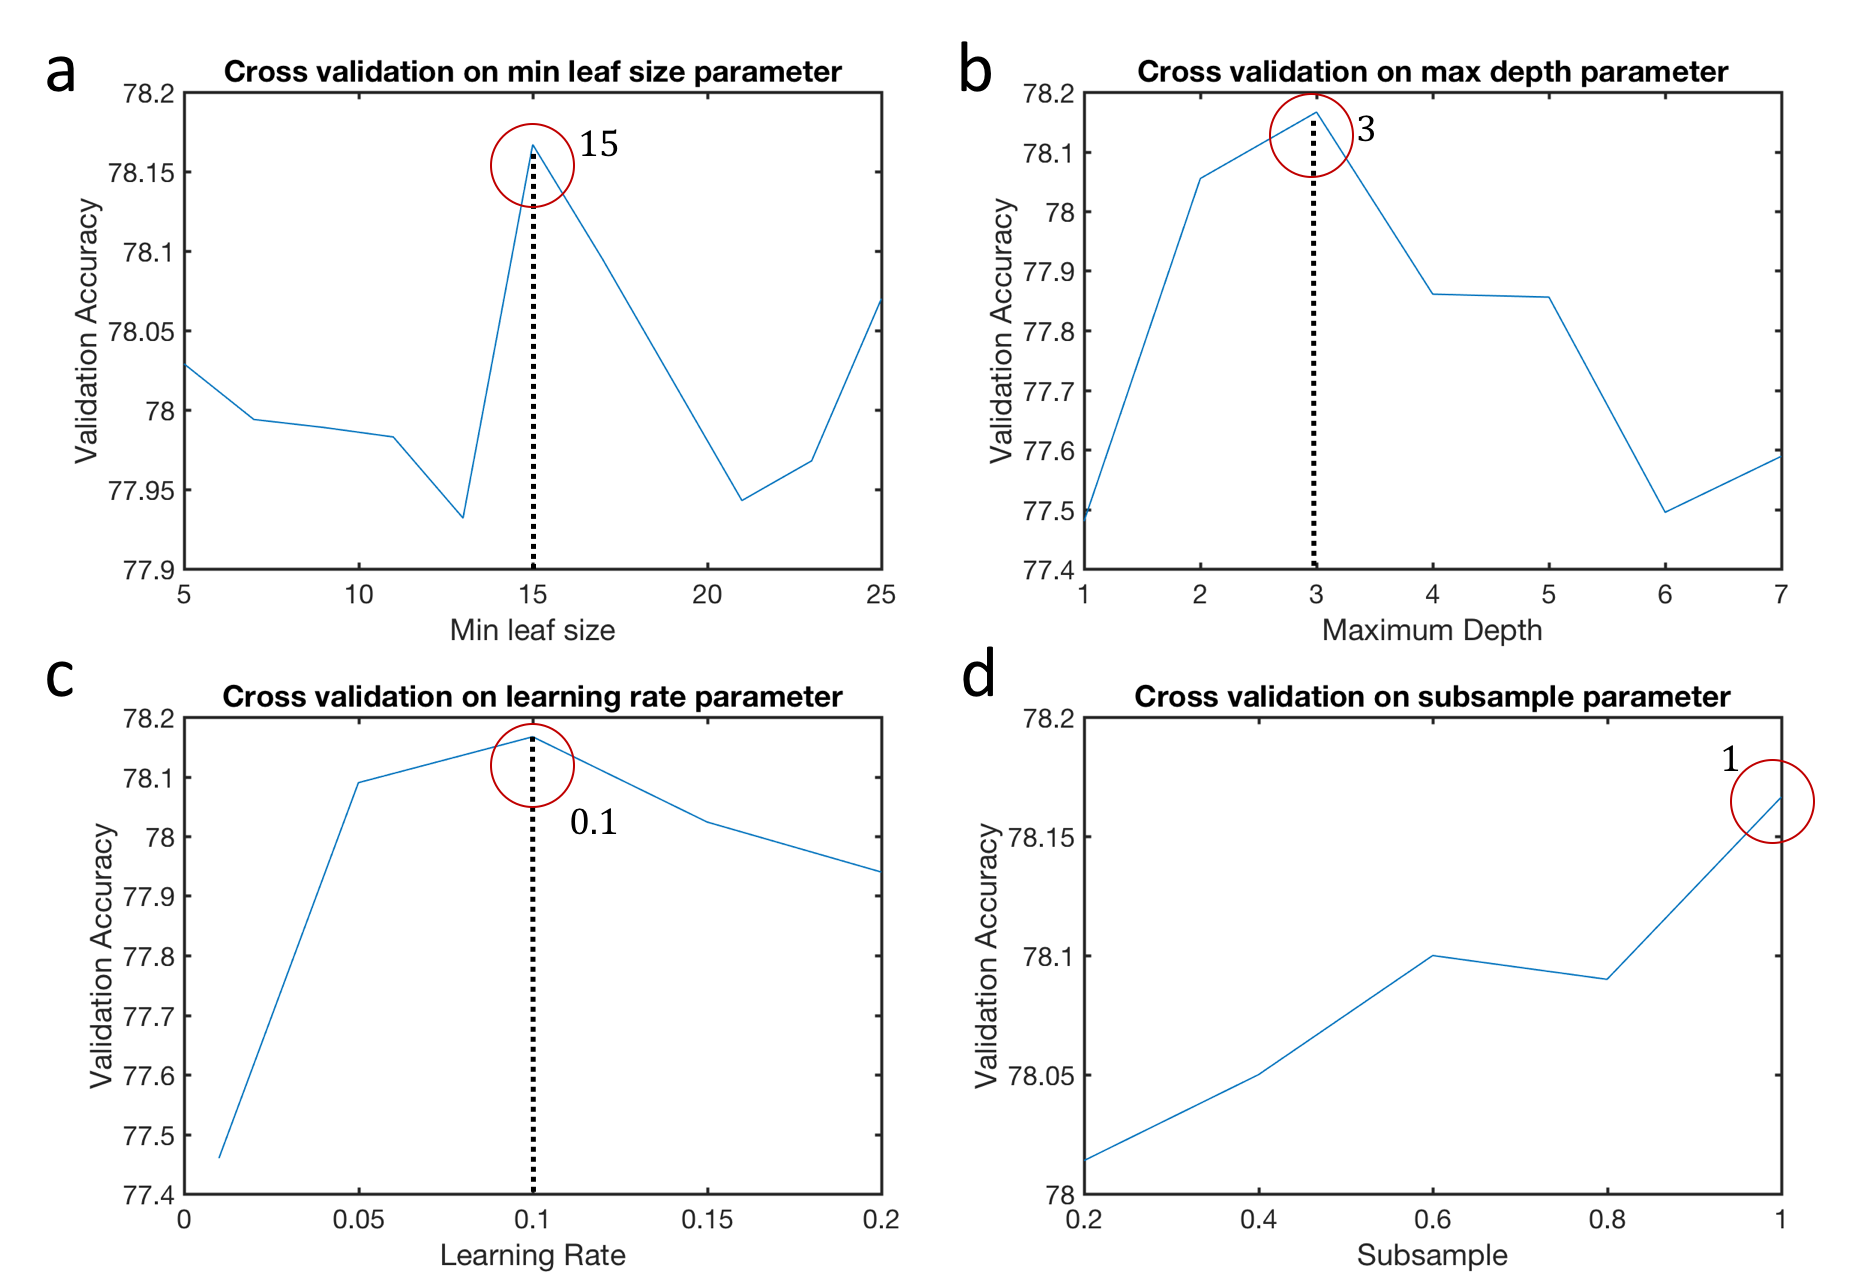
\includegraphics[scale=0.4]{figure3/figure3.png}
\caption{\textbf{Cross validation for model parameter selection} \textit{Through an exhaustive grid search we determined the quadruple of parameters which gave the best validation accuracy around $78.2\%$. (a) Validation on min leaf size shows a peak at 15 (b) Validation on max depth shows peak at 3 (c) Validation on learning rate shows a peak at 0.1 (d) Validation on subsample shows a peak at 1}}
\end{figure}


\newpage
\subsubsection*{[iii]. Handling class-imbalance}
Upon analyzing the label distribution of the training data, we found that over $73\%$ were of class $1$, while only $27\%$ were class 2. Such class-imbalance can often lead to the tree predicting in favor of the majority class, which generates a low-precision, high-recall classifier. (In terms of the majority class) Our solution to tackling this class-imbalance problem was to set a prediction bias. To elaborate, first recall that a decision tree makes predictions by taking the argmax of the probability distribution over the class-labels at each leaf node. For a binary classification task, this means that the class with probability higher than 0.5 becomes the prediction. We instead modify the threshold with a prediction bias $p$ such that in order for class 1 to be the prediction at a leaf node, it must have a probability $0.5 + p$. Fig. 4. shows cross validation accuracy while varying $p$ from $-0.02$ to $0.02$. Other bias values ($> 0.2$ or $< -0.2$) led to worse model performance than the optimum value $p = 0.013$.
\begin{figure}[h]
\center
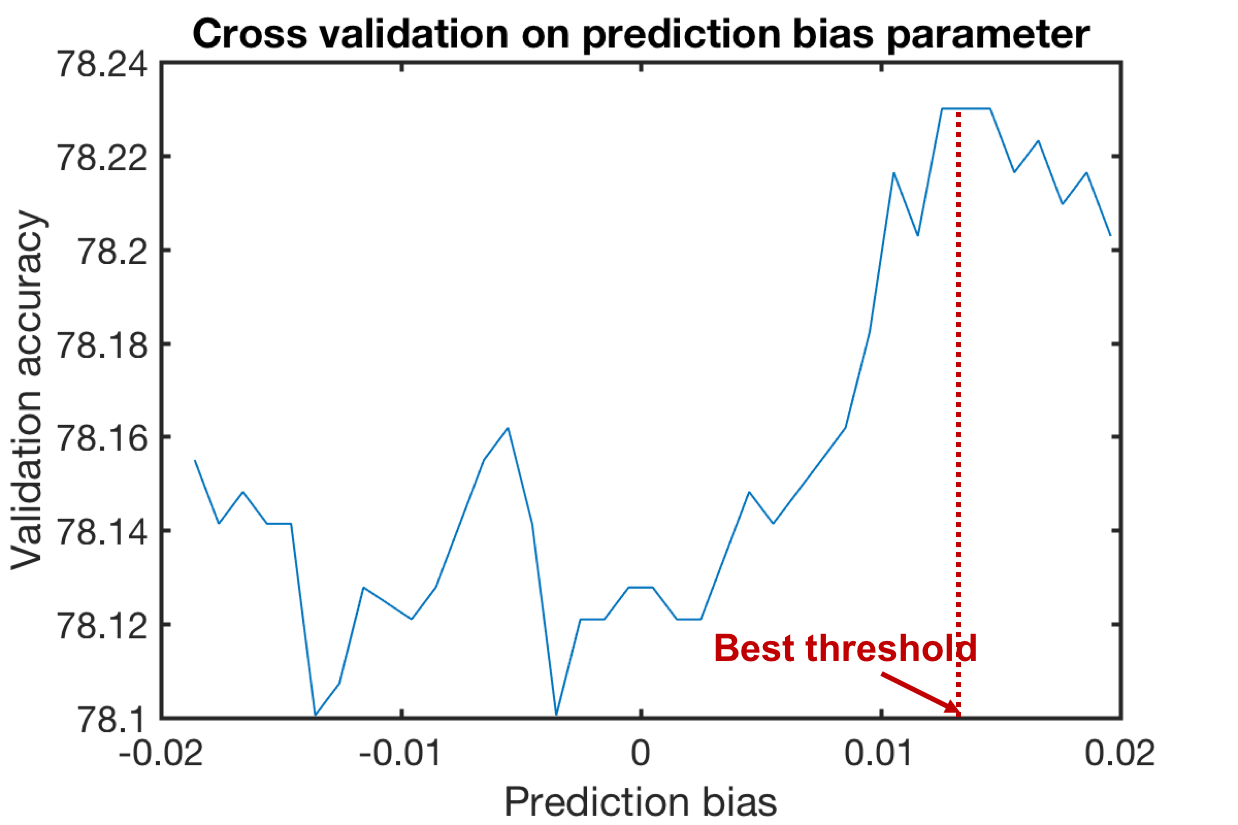
\includegraphics[scale=0.5]{figure4/figure4.png}
\caption{\textbf{Cross validation accuracy vs prediction bias} \textit{Validation accuracy is highest with a prediction bias of $0.013$. Qualitatively, a positive prediction bias means to predict in favor of class 2 (minority class). }}
\end{figure}

\subsubsection*{[iv]. Ensemble selection}
$85\%$ of the total training data was partitioned towards training a model library and $15\%$ was reserved as a validation set to ensemble select on. We trained a model library consisting of $20$ GBMs, $20$ ANNs, and $20$ Random Forests. Upon an initial attempt of building a library with only GBMs, we realized that boosting methods have very low variance. Hence, most models generated similar predictions and ensemble selection did not lead to an improvement in the validation accuracy. Hence, we decided to add more diverse models into the pool in order to take the full benefit of both bagging and boosting. For succinctness of the report, we omit the parameter optimization process for ANNs and RFs. The final accuracy of the ensemble selected model was approximately $0.1$ better than a single GBM attaining the highest validation accuracy $\approx 78.3$. Our submission of this model received a \textbf{final score of 78.7 on the 2008 dataset and 76.17 on the 2012 dataset}.

\newpage

\section*{4. Conclusion}
\subsubsection*{[i]. Overall rank: $9^{th}$ for 2008 dataset, $26^{th}$ for 2012 dataset}

\subsubsection*{[ii]. Challenges}
Dealing with real-word data was more difficult than training models to fit low-noise data which are often given out for homework assignments. We believe that learning how to engineer the features effectively was the most challenging aspect of this project. This required us to understand the features beyond their numeric values, which required many hours because there were 380 of them. We learned that many feature engineering techniques are task specific which led to many of our initial attempts (such as PCA, Univariate selection) failing. Through overcoming these challenges, the most important lesson that we learned was that it is crucial to fully understand the data before attempting any feature selection or model optimization.

\subsubsection*{[iii]. Concluding Remarks}
This competition gave us a sense of the difficulties machine learning practitioners face when modeling noisy real-word data. Lastly and most importantly, we would like to thank the TAs and the instructor for organizing such a great learning experience. We hope our report demonstrates that your efforts to find creative ways in teaching were not in vein.

















\end{document}
